\chapter{Diskussion}\label{cha:fazit}
Die ursprüngliche Frage dieser Arbeit lautete, wie genau wird das Ergebnis einer Elementarladung ausfällt, wenn das Experiment, das vor über hundert Jahren entwickelt wurde, heute wiederholt wird. Die Antwort darauf ist, verblüffend genau. Mithilfe eines Experimentierkasten wurde ein Endergbnis erzielt, welches 3.22\% abweicht vom Literaturwert. Dies beantwortet die Frage, dass die Ergebnisse dieses Experiments heute genau oder genauer ausfallen.

Zu Beginn wurde davon ausgegangen, dass die Messergebnisse eines solchen Experiments stark ausschwanken würden und nie in der Grössenordnung der Elementarladung liegen werden. Wiederlegt, wurde diese Erwartung, durch das Auswerten der Messergebnisse. Die ersten Auswertungen waren falsch. Es lag an den falschen Grössenordnungen der Messungen. Beispielsweise wurde das $10^{-5}$ vergessen beim ablesen der Luftviskosität oder die Einheit $mm/s$ wurde nicht in $m/s$ umgerechnet. Bei 12 verschiedenen Grössen konnten am Anfang mehrere Falsch sein, dies führte dazu, dass die Endresultate nicht stimmten.

Diese Arbeit behandelt ausschliesslich die Genauigkeit dieses Experiments. Mit diesem Ergebnis kann nicht einene neuen Wert der Elementarladung festgelegt werden. Dafür wären mehr Messreihen und andere Methoden zur experimentellen Bestimmung, welche dieses Ergebnis bestätigten, notwendig gewesen. 

Eine solche Genauigkeitsüberprüfung könnte bei anderen älteren Experimenten vorgenommen werden. Eine weitere Forschung wäre zum Beispiel, die Elementarladung theoretisch zu bestimmen und das Ergebnis dann mit einer experimentellen Bestimmung zu vergleichen.

Alle Schwierigkeiten, die während dem Experimentieren auftauchten, konnten mit der Zeit behoben werden. Beim dritten Anlauf kamen zum ersten Mal brauchbare Endresultate heraus. 

\section{Methoden}\label{sec:methoden}
Dieses Experiment erfordert viel Geduld und Präzision. Das grösste Problem lag an den Berechnungen. Eine komplexe Formel und gleichzeitig etwa 40 verschiedene Messungen, die verarbeitet werden mussten. Wie kann dieser Prozess vereinfacht und währenddessen Zeit effizienter genutzt werden? Die Antwort darauf liegt in der Programmierung. Für Berechnungen der Ergebnisse wurde Python verwendet. Mit dem Pandas-Modul konnten Daten aus Excel-Tabellen gelesen, verarbeitet und wieder zurückgeschrieben werden \parencite[vgl.]{Inc_2024}. 
Da diese Arbeit in \LaTeX~geschrieben wurde, mussten alle Grafiken von .png in .pdf Format konvertiert werden. Dieser Schritt übernahm ein Python-Skript. Die Fallzeiten konnten mithilfe eines Assistenten aufgezeichnet werden. Dies ergab am Schluss einen grösseren Fehler bei den Fall- und Steigzeiten, mit einer Stoppuhr hätte man das aktuelle Tröpfchen verloren, da man das Auge vom Mikroskop wegnehmen muss, um die Zeit abzulesen. 

\begin{figure}[h]
	\centering
	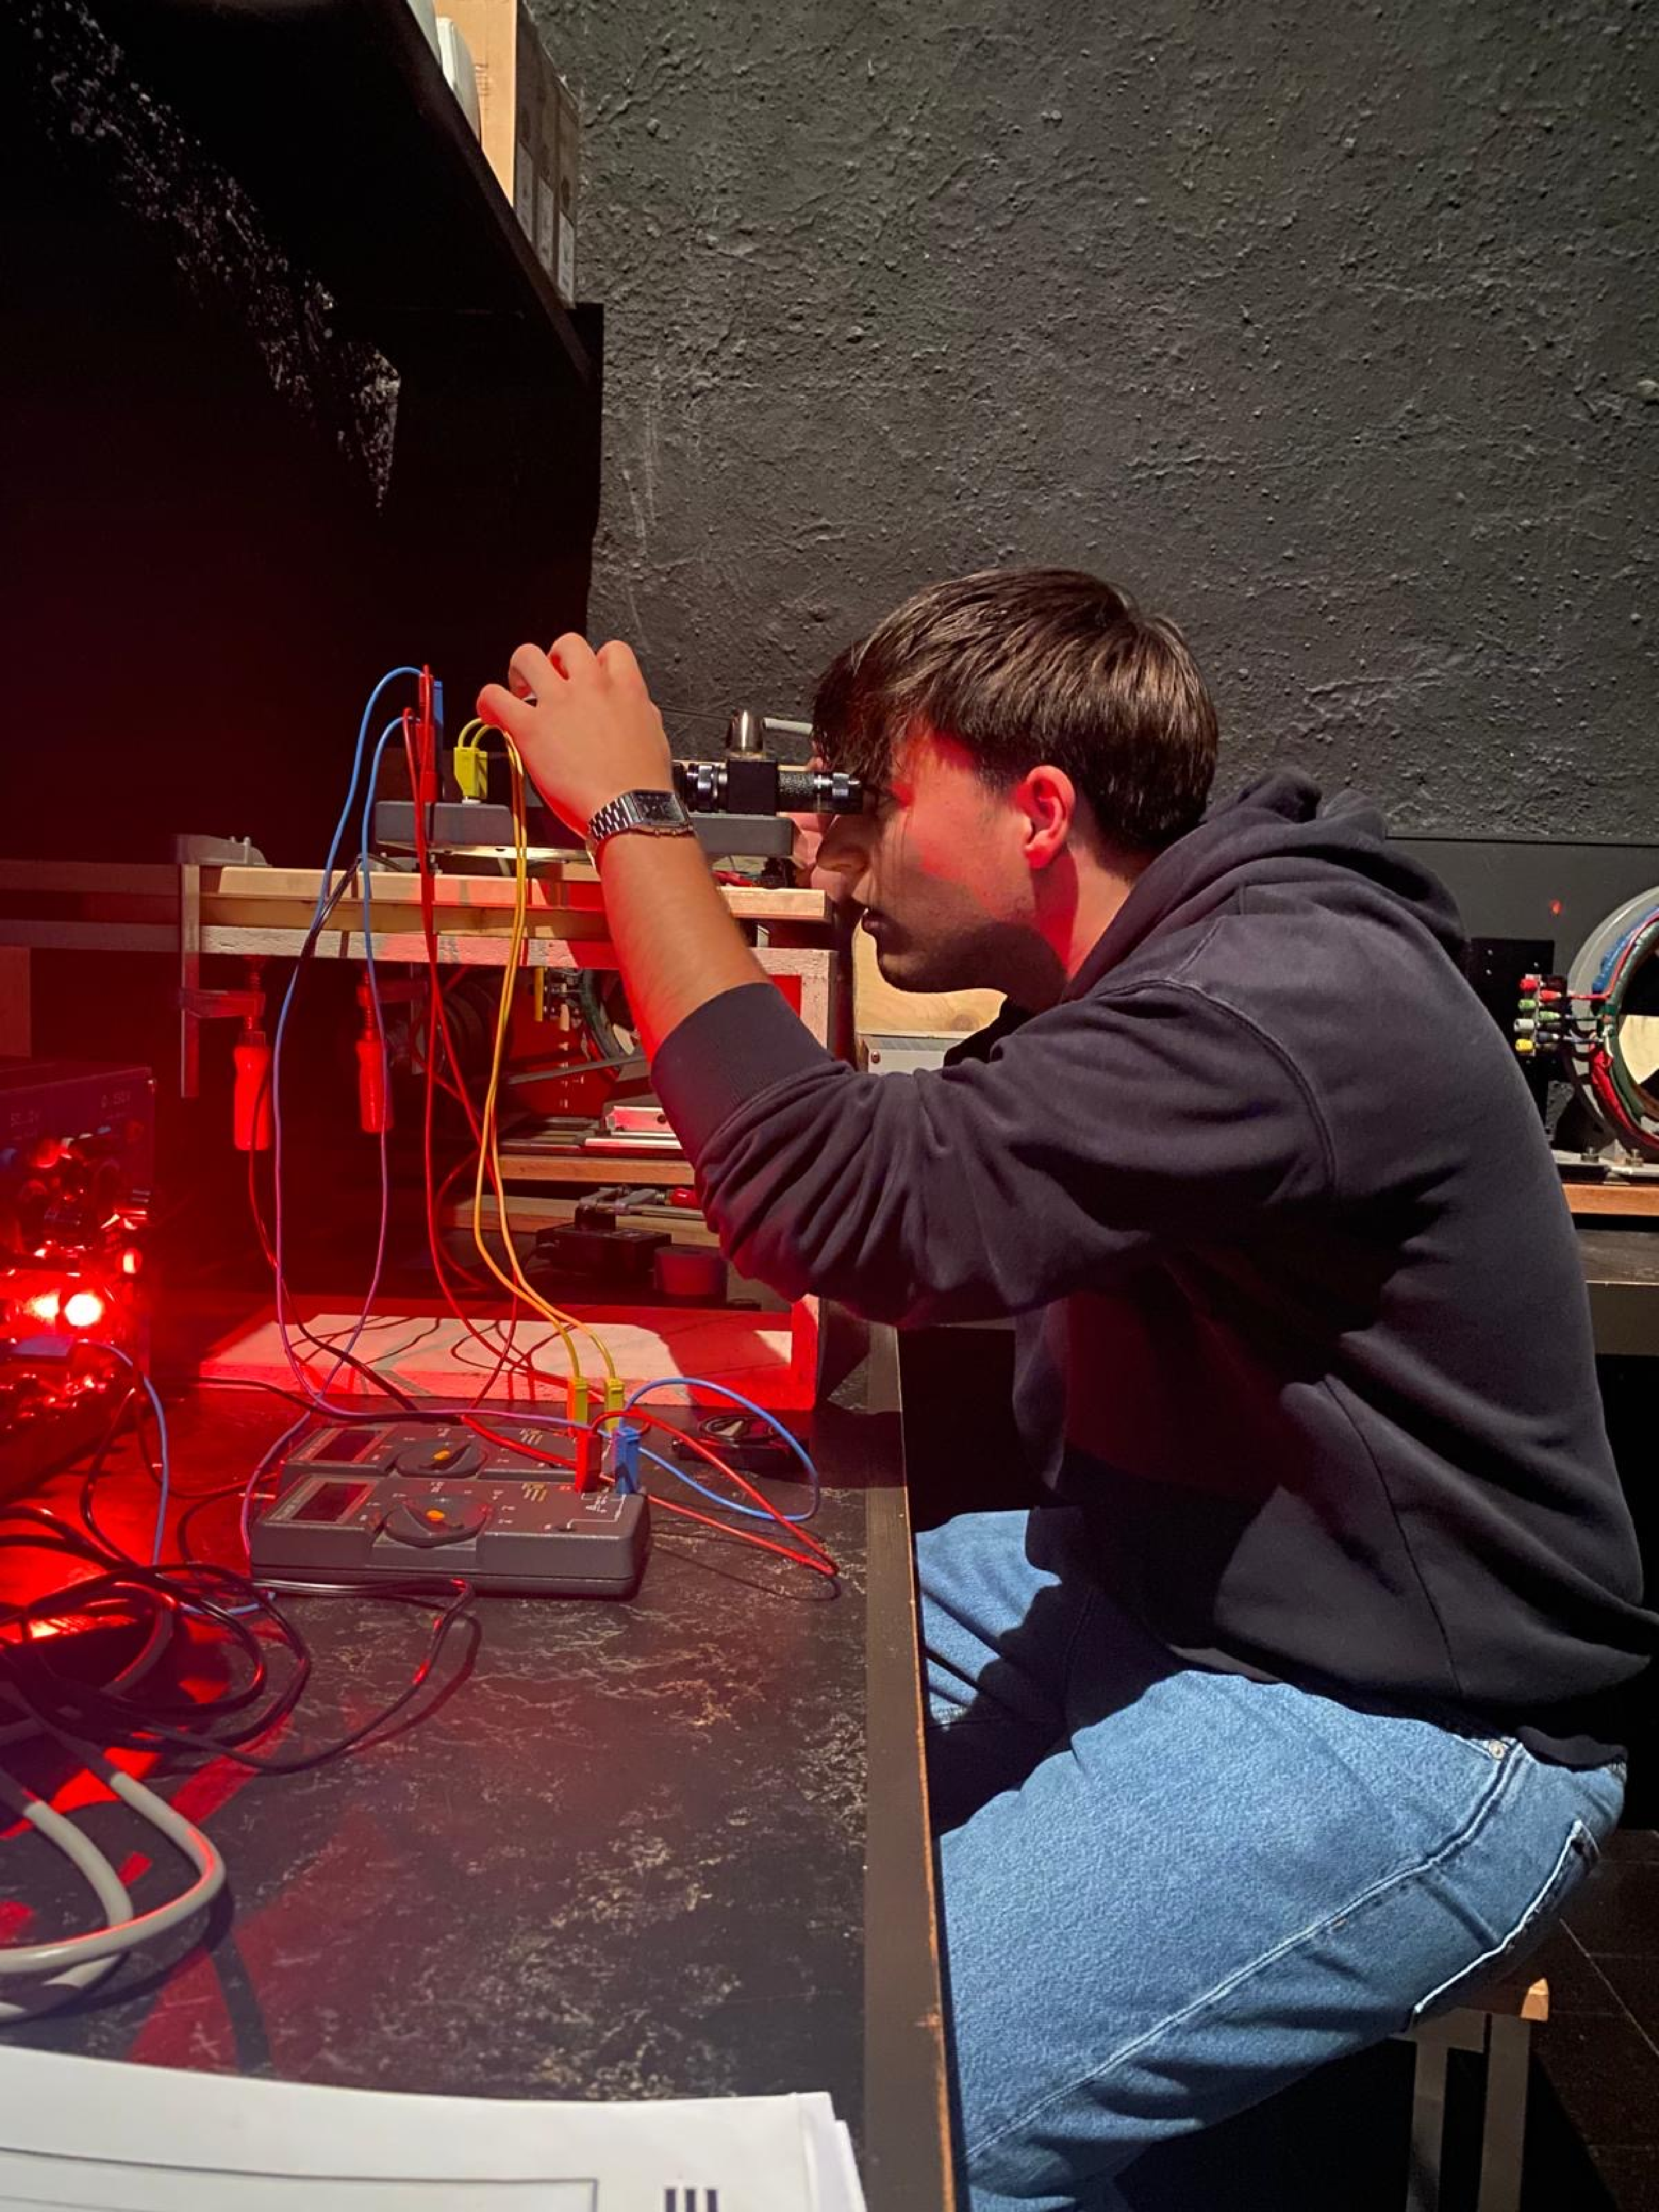
\includegraphics[scale=0.25]{bilder/pdf/bildExperimentieren.pdf}
	\caption{Samuel während dem Experimentieren}
	\label{fig:experimentieren}
\end{figure}